% Options for packages loaded elsewhere
\PassOptionsToPackage{unicode}{hyperref}
\PassOptionsToPackage{hyphens}{url}
\PassOptionsToPackage{dvipsnames,svgnames*,x11names*}{xcolor}
%
\documentclass[
  10pt,
  spanish,
]{book}
\usepackage{amsmath,amssymb}
\usepackage{lmodern}
\usepackage{ifxetex,ifluatex}
\ifnum 0\ifxetex 1\fi\ifluatex 1\fi=0 % if pdftex
  \usepackage[T1]{fontenc}
  \usepackage[utf8]{inputenc}
  \usepackage{textcomp} % provide euro and other symbols
\else % if luatex or xetex
  \usepackage{unicode-math}
  \defaultfontfeatures{Scale=MatchLowercase}
  \defaultfontfeatures[\rmfamily]{Ligatures=TeX,Scale=1}
\fi
% Use upquote if available, for straight quotes in verbatim environments
\IfFileExists{upquote.sty}{\usepackage{upquote}}{}
\IfFileExists{microtype.sty}{% use microtype if available
  \usepackage[]{microtype}
  \UseMicrotypeSet[protrusion]{basicmath} % disable protrusion for tt fonts
}{}
\makeatletter
\@ifundefined{KOMAClassName}{% if non-KOMA class
  \IfFileExists{parskip.sty}{%
    \usepackage{parskip}
  }{% else
    \setlength{\parindent}{0pt}
    \setlength{\parskip}{6pt plus 2pt minus 1pt}}
}{% if KOMA class
  \KOMAoptions{parskip=half}}
\makeatother
\usepackage{xcolor}
\IfFileExists{xurl.sty}{\usepackage{xurl}}{} % add URL line breaks if available
\IfFileExists{bookmark.sty}{\usepackage{bookmark}}{\usepackage{hyperref}}
\hypersetup{
  pdftitle={Diseño y análisis estadístico en las encuestas de hogares de América Latina},
  pdfauthor={Andrés Gutiérrez},
  pdflang={es},
  colorlinks=true,
  linkcolor=blue,
  filecolor=Maroon,
  citecolor=Blue,
  urlcolor=Blue,
  pdfcreator={LaTeX via pandoc}}
\urlstyle{same} % disable monospaced font for URLs
\usepackage{longtable,booktabs,array}
\usepackage{calc} % for calculating minipage widths
% Correct order of tables after \paragraph or \subparagraph
\usepackage{etoolbox}
\makeatletter
\patchcmd\longtable{\par}{\if@noskipsec\mbox{}\fi\par}{}{}
\makeatother
% Allow footnotes in longtable head/foot
\IfFileExists{footnotehyper.sty}{\usepackage{footnotehyper}}{\usepackage{footnote}}
\makesavenoteenv{longtable}
\usepackage{graphicx}
\makeatletter
\def\maxwidth{\ifdim\Gin@nat@width>\linewidth\linewidth\else\Gin@nat@width\fi}
\def\maxheight{\ifdim\Gin@nat@height>\textheight\textheight\else\Gin@nat@height\fi}
\makeatother
% Scale images if necessary, so that they will not overflow the page
% margins by default, and it is still possible to overwrite the defaults
% using explicit options in \includegraphics[width, height, ...]{}
\setkeys{Gin}{width=\maxwidth,height=\maxheight,keepaspectratio}
% Set default figure placement to htbp
\makeatletter
\def\fps@figure{htbp}
\makeatother
\setlength{\emergencystretch}{3em} % prevent overfull lines
\providecommand{\tightlist}{%
  \setlength{\itemsep}{0pt}\setlength{\parskip}{0pt}}
\setcounter{secnumdepth}{5}
\usepackage{setspace}
%\linespread{1.5}
%\usepackage{tikz}
%\usetikzlibrary{shapes,arrows}
\usepackage{pdflscape}
\newcommand{\blandscape}{\begin{landscape}}
\newcommand{\elandscape}{\end{landscape}}
\renewcommand{\thesection}{\Roman{section}}
\renewcommand{\thesubsection}{\Alph{subsection}}
\usepackage{booktabs}
\usepackage{amsthm}
\makeatletter
\def\thm@space@setup{%
  \thm@preskip=8pt plus 2pt minus 4pt
  \thm@postskip=\thm@preskip
}
\makeatother
\ifxetex
  % Load polyglossia as late as possible: uses bidi with RTL langages (e.g. Hebrew, Arabic)
  \usepackage{polyglossia}
  \setmainlanguage[]{spanish}
\else
  \usepackage[main=spanish]{babel}
% get rid of language-specific shorthands (see #6817):
\let\LanguageShortHands\languageshorthands
\def\languageshorthands#1{}
\fi
\ifluatex
  \usepackage{selnolig}  % disable illegal ligatures
\fi
\usepackage[]{natbib}
\bibliographystyle{apalike}

\title{Diseño y análisis estadístico en las encuestas de hogares de América Latina}
\author{Andrés Gutiérrez\footnote{Experto regional en estadísticas sociales - Unidad de Estadística Social - Comisión Económica para América Latina y el Caribe (CEPAL) - \href{mailto:andres.gutierrez@cepal.org}{\nolinkurl{andres.gutierrez@cepal.org}}}}
\date{2021-06-14}

\begin{document}
\maketitle

{
\hypersetup{linkcolor=}
\setcounter{tocdepth}{1}
\tableofcontents
}
\listoftables
\listoffigures
\hypertarget{prefacio}{%
\chapter*{Prefacio}\label{prefacio}}
\addcontentsline{toc}{chapter}{Prefacio}

\begin{figure}

\includegraphics[width=100px]{Pics/CClicence} \caption{Licencia de Creative Commons}\label{fig:unnamed-chunk-1}
\end{figure}

La versión online de este libro está licenciada bajo una \href{http://creativecommons.org/licenses/by-nc-sa/4.0/}{Licencia Internacional de Creative Commons para compartir con atribución no comercial 4.0}.

\hypertarget{resumen}{%
\chapter*{Resumen}\label{resumen}}
\addcontentsline{toc}{chapter}{Resumen}

Las encuestas de hogares son un instrumento necesario para realizar seguimiento a un conjunto amplio de indicadores requeridos para el diseño y evaluación de las políticas públicas. Las encuestas de hogares que se implementan en América Latina son de tipo y características diversas. Aunque los conceptos y procesos para su diseño y análisis guardan similitudes, este documento se enfoca principalmente en los procesos referidos a las encuestas de empleo y de propósitos múltiples, con las que los países estiman los principales indicadores relacionados con el mercado laboral, el nivel y distribución de ingresos y la condición de pobreza y las principales características sociodemográficas de la población. Se realiza un recorrido por los diferentes diseños de muestreo, las metodologías más usadas en la selección de las muestras y las estrategias de estimación de los parámetros de interés. También se revisan las técnicas utilizadas para medir el error de muestreo y los métodos disponibles para encarar desafíos como la ausencia de respuesta y la desactualización de los marcos de muestreo.

\textbf{UNBIS Keywords}. Encuestas por muestreo, encuestas de hogares, indicadores socioeconómicos.

\hypertarget{introducciuxf3n}{%
\chapter{Introducción}\label{introducciuxf3n}}

Las encuestas de hogares son un caso particular de investigación social que indaga acerca de características específicas a nivel del individuo, del hogar o de la vivienda, con el fin de obtener inferencias precisas acerca de constructos de interés. Por su naturaleza, estas investigaciones están relacionadas con variables de salud, educación, ingresos, gastos, situación laboral, acceso y uso de servicios, entre muchas otras. En algunas ocasiones, las encuestas de hogares tienen como objetivo la estimación de uno o varios indicadores que resumen un constructo económico o social. Sin embargo, existe una tendencia creciente de extender las encuestas a constructos más diversos. Es así como cada vez tienen más espacio las encuestas de propósitos múltiples como una fuente relevante de información que permite monitorear indicadores sociales.

En este tipo de encuestas, el hogar es la unidad de análisis, la cual ha sido definida por la División de Estadística de la Organización de las Naciones Unidas \citep{United-Nations_2011} como:

\begin{quote}
\begin{enumerate}
\def\labelenumi{\alph{enumi}.}
\tightlist
\item
  Un grupo de dos o más personas que se combinan para ocupar la totalidad o parte de una vivienda y para proporcionarse alimentos y posiblemente otros artículos esenciales para la vida. El grupo puede estar compuesto solo de personas relacionadas o de personas no relacionadas o de una combinación de ambos. El grupo también puede compartir sus ingresos.
\item
  Una persona que vive sola en una vivienda separada o que ocupa, como huésped, una habitación (o habitaciones) separada de una vivienda pero que no se une a ninguno de los otros ocupantes de la vivienda para formar parte de una hogar de múltiples personas.
\end{enumerate}
\end{quote}

Nótese que la anterior definición refleja la dinámica natural del cambio en las poblaciones de hogares, por lo cual se deben tener distintos enfoques para abordar el problema de la medición de indicadores sociales. En América Latina, existen una gran variedad de encuestas que abordan diferentes problemáticas sociales. Todas y cada una de ellas han sido diseñadas cuidadosamente para que respondan a las necesidades de la sociedad. Este documento plantea una recopilación de las técnicas usadas tanto en su diseño, como en su análisis.

No todas las encuestas se diseñan de la misma forma y por ende debe haber una distinción entre ellas. Por ejemplo, \citet{Kalton_Citro_1993} afirman que las encuestas de hogares pueden clasificarse en varios tipos:

\begin{itemize}
\tightlist
\item
  \emph{Encuestas repetidas}, definidas como una serie de encuestas transversales aplicadas en diferentes momentos del tiempo con el mismo diseño metodológico, en donde la selección de hogares se hace de forma independiente para cada aplicación.
\item
  \emph{Encuestas tipo panel}, para las cuales los datos son recolectados en diferentes momentos del tiempo utilizando la misma muestra de hogares en el tiempo.
\item
  \emph{Encuestas rotativas}, en donde un porcentaje de hogares se mantiene en un periodo de tiempo respondiendo la encuesta y en cada aplicación algunos hogares son reemplazados por nuevos hogares de forma planificada.
\end{itemize}

El diseño de la encuesta dependerá sistemáticamente del objetivo de la medición. Por ejemplo, \citet{Kalton_2009} afirma que es prudente hacer un buena inversión en el desarrollo e implementación de un buen diseño para amortizar los costos de todo el estudio. Por lo tanto, lo que se quiere al diseñar una encuesta de hogares es que sea un instrumento confiable, que brinde estimaciones exactas y precisas, puesto que de lo contrario no se podrían monitorear las políticas públicas y los indicadores de interés de forma consistente. Por ejemplo, uno de los indicadores sociales con mayor impacto es la tasa de desocupación, que mide la razón entre la cantidad de personas que se encuentran desocupados, pero que forman parte del mercado de trabajo. Las encuestas de empleo tienen características particulares, diferentes a las de las encuestas que miden otro tipo de constructos. \citet{Duncan_Kalton_1987} mencionan que las encuestas de hogares pueden proveer estimaciones de los parámetros poblacionales en distintos puntos del tiempo, por ejemplo, la estimación de la tasa de desocupación mensual; proveer estimaciones del cambio neto de los parámetros poblacionales entre periodos de tiempo, por ejemplo, el cambio en la tasa de desocupación entre dos periodos consecutivos; o incluso medir varios componentes de cambio individual, por ejemplo cambios brutos en la situación laboral de los jefes de hogar, para lo cual se requiere que la encuesta contemple un diseño de panel o de panel rotativo.

La medición de los indicadores en el mercado de trabajo es sólo un pequeño componente en el basto universo de posibilidades de medición que brindan las encuestas de hogares. Por esta razón, este tipo de levantamientos se ha convertido en una herramienta fundamental para medir indicadores sociales en todo el mundo y que, en particular, permiten que las naciones de América Latina puedan hacer seguimiento a su desarrollo económico y social. Sin embargo, este tipo de instrumentos puede ser utilizado como herramienta para monitorear el progreso de los países en términos de metas y objetivos comunes. Es así como en 2015, la Asamblea General de la Organización de las Naciones Unidas aprobó una resolución que plantea un plan de acción en favor de las personas, el planeta y la prosperidad \citep{United_Nations_2015}. Esa resolución propone el seguimiento de 17 Objetivos de Desarrollo Sostenible (\href{https://sustainabledevelopment.un.org}{ODS}) y 169 metas de carácter integrado e indivisible que se conjugan en las dimensiones económica, social y ambiental. Para realizar el seguimiento a los ODS es posible utilizar diferentes fuentes de información, como censos, registros administrativos, registros estadísticos, proyecciones demográficas y también las encuestas de hogares \citep{United_Nations_2016}. En particular, cada una de las metas de los ODS contiene indicadores, muchos de los cuales no pudieran ser estimados de no ser por la información disponible en las encuestas de hogares.

Por ejemplo, el objetivo \textbf{8} busca \emph{promover el crecimiento económico sostenido, inclusivo y sostenible, el empleo pleno y productivo y el trabajo decente para todos}. Claramente de este objetivo se desprenden indicadores que permiten conocer la evolución de los países en la consecución de las metas. Dentro de este objetivo, se encuentra la meta \textbf{8.6} que apunta a reducir sustancialmente la proporción de jóvenes sin empleo y sin educación o entrenamiento. Esta meta se mide con el indicador \textbf{8.6.1} definido como la proporción de jóvenes (entre 15 y 24 años de edad) sin educación y sin empleo.

Desde otra perspectiva, en el marco de la decimotercera conferencia internacional de estadísticos del trabajo en 1982, la Organización Internacional del Trabajo (OIT) adoptó algunas directrices concernientes con la medición y análisis de estadísticas oficiales de la fuerza de trabajo, del empleo y del desempleo con miras a mejorar la comparabilidad de las cifras y mejorar su utilidad en los países \citep{OIT_1982}. En esta resolución se hace un énfasis especial en que las encuestas de hogares constituyen un medio apropiado de recopilación de datos sobre la población económicamente activa y que la planeación de estas investigaciones en los países debería ceñirse a las normas internacionales. Por consiguiente, la resolución afirma que las encuestas de hogares deberían:

\begin{enumerate}
\def\labelenumi{\arabic{enumi}.}
\tightlist
\item
  Brindar datos de la población económicamente activa.
\item
  Proveer estadísticas básicas de sus actividades durante el año, así como las relaciones entre el empleo, ingreso y otras características económicas y sociales.
\item
  Proveer datos sobre otros temas particulares para responder a las necesidades a largo plazo y de índole permanente.
\end{enumerate}

En el año 2013, la OIT decidió revisar esta resolución y propuso algunos cambios en el marco de la 19 Conferencia Internacional de Estadísticos del Trabajo en donde se acogieron algunas modificaciones en términos de los objetivos de medición y el alcance de los sistemas nacionales de estadísticas del trabajo, el concepto de trabajo en todas sus formas, el empleo, la medición de las personas en situación de subutilización de la fuerza de trabajo, métodos de recopilación de datos, entre otras \citep{OIT_2013}. Es así como los Institutos Nacionales de Estadística (INE) de América Latina no sólo planean las encuestas de hogares de tal forma que puedan responder a los nuevos retos en términos de la estimación de los parámetros de interés en cuento al trabajo remunerado o no remunerado para mantener la comparabilidad de las estadísticas laborales entre los países proporcionando nuevos y mejores indicadores para contribuir al análisis de la dinámica del mercado laboral, sino que se actualizan paulatinamente para poder brindar la información que la sociedad necesita a medida que evoluciona el constructo social de interés.

Es importante resaltar que los indicadores de bienestar (en términos de ingresos y gastos) también hacen parte del conjunto de parámetros que se pueden estimar desde las encuestas de hogares. Medir el ingreso a partir de las encuestas de hogares se constituye en un reto metodológico para los institutos nacionales de estadística en el mundo, y particularmente en América Latina. Es recomendable seguir las directrices de la Comisión Económica para Europa que revisten una actualización de los estándares internacionales, recomendaciones y buenas prácticas en la medición del ingreso en los hogares. Por ejemplo, el llamado Grupo de Canberra ha revisado exhaustivamente el tópico de la estimación del ingreso estudiando las prácticas de algunos países en términos del aseguramiento de la calidad y la publicación de este tipo de estadísticas oficiales y ha provisto la siguiente definición de ingreso en el hogar \citep{United-Nations_2011}:

\begin{quote}
\emph{El ingreso del hogar se compone de las entradas monetarias, en especie o en servicios que por lo general son frecuentes y regulares, están destinadas al hogar o a los miembros del hogar por separado y se reciben a intervalos anuales o con mayor frecuencia. Durante el período de referencia en el que se reciben, tales entradas están potencialmente disponibles para el consumo efectivo y, habitualmente, no reducen el patrimonio neto del hogar.}
\end{quote}

Con base en lo anterior, el uso de las encuestas de hogares para estimar el ingreso reviste retos metodológicos mayores puesto que los entrevistados deben responder con precisión cuando se les indague por este constructo que contiene los ingresos personales de cada individuo en el hogar, como sueldos y salarios, ganancias, ingresos del empleo, pensiones, etc. y también los ingresos del hogar, incluidas las rentas por alquiler y los ingresos generados por el comercio. Por lo tanto, el diseño de la encuesta debe tener en cuenta la definición de un instrumento que sea relevante para el respondiente y le permita identificar y, en algunas ocasiones, recordar la información con un cierto grado de exactitud. Por ejemplo, si el respondiente es empleado regular, el instrumento de medición debería planearse de tal manera que el entrevistado pueda recordar información de interés, como los rubros de seguridad social hechos por su empleador. Por otro lado, si se requiere que el respondiente brinde información acerca de un determinado periodo de tiempo, el planteamiento de la pregunta, la forma de indagar y el entrenamiento de los encuestadores pueden sesgar sistemáticamente la respuesta y por consiguiente inducir estimaciones poco confiables. Mucho se ha investigado al respecto de cómo realizar preguntas certeras en este tipo de levantamientos y el lector interesado puede consultar los trabajos de \citet{Biemer_Lyberg_2003}, \citet{Presser_Rothgeb_Couper_Lessler_Martin_Martin_Singer_2004}, y \citet{Groves_Fowler_Couper_Lepkowski_Singer_Tourangeau_2009}.

Este documento pretende revisar algunas de las metodologías más usadas por los INE de América Latina en cuanto al diseño y análisis estadístico de las encuestas de hogares y puede servir de guía técnica a los estadísticos de la región involucrados en los proceso técnicos de este tipo de encuestas. De la misma forma, este documento considera conjuntamente los dos principales momentos de las encuestas: el diseño y el análisis. Nótese que estos momentos están escindidos por el levantamiento de la información en campo y parten la realización de la encuesta en dos. Los lectores que están familiarizados con la investigación social a través de las encuestas de hogares encontrarán que las encuestas se planean teniendo en cuenta muchos pormenores que podrían suceder en campo, pero que este diseño en la mayoría de ocasiones toma distancia de la información que se recolecta en campo. Es por esto que el trabajo de las encuestas asciende cuando se logra plasmar la información en forma de base de datos. En este segundo momento es cuando se debe asegurar que lo que se planificó efectivamente sea incorporado en el análisis de esta información. Desde esta perspectiva, este documento puede verse en dos partes: los capítulos 2, 3 y 4 abordan el diseño, mientras que los capítulos 4, 5 y 6 y 7 abordan el análisis. Esta distinción así como los procesos que la componen se presenta en la Figura 1.

\begin{figure}
\centering
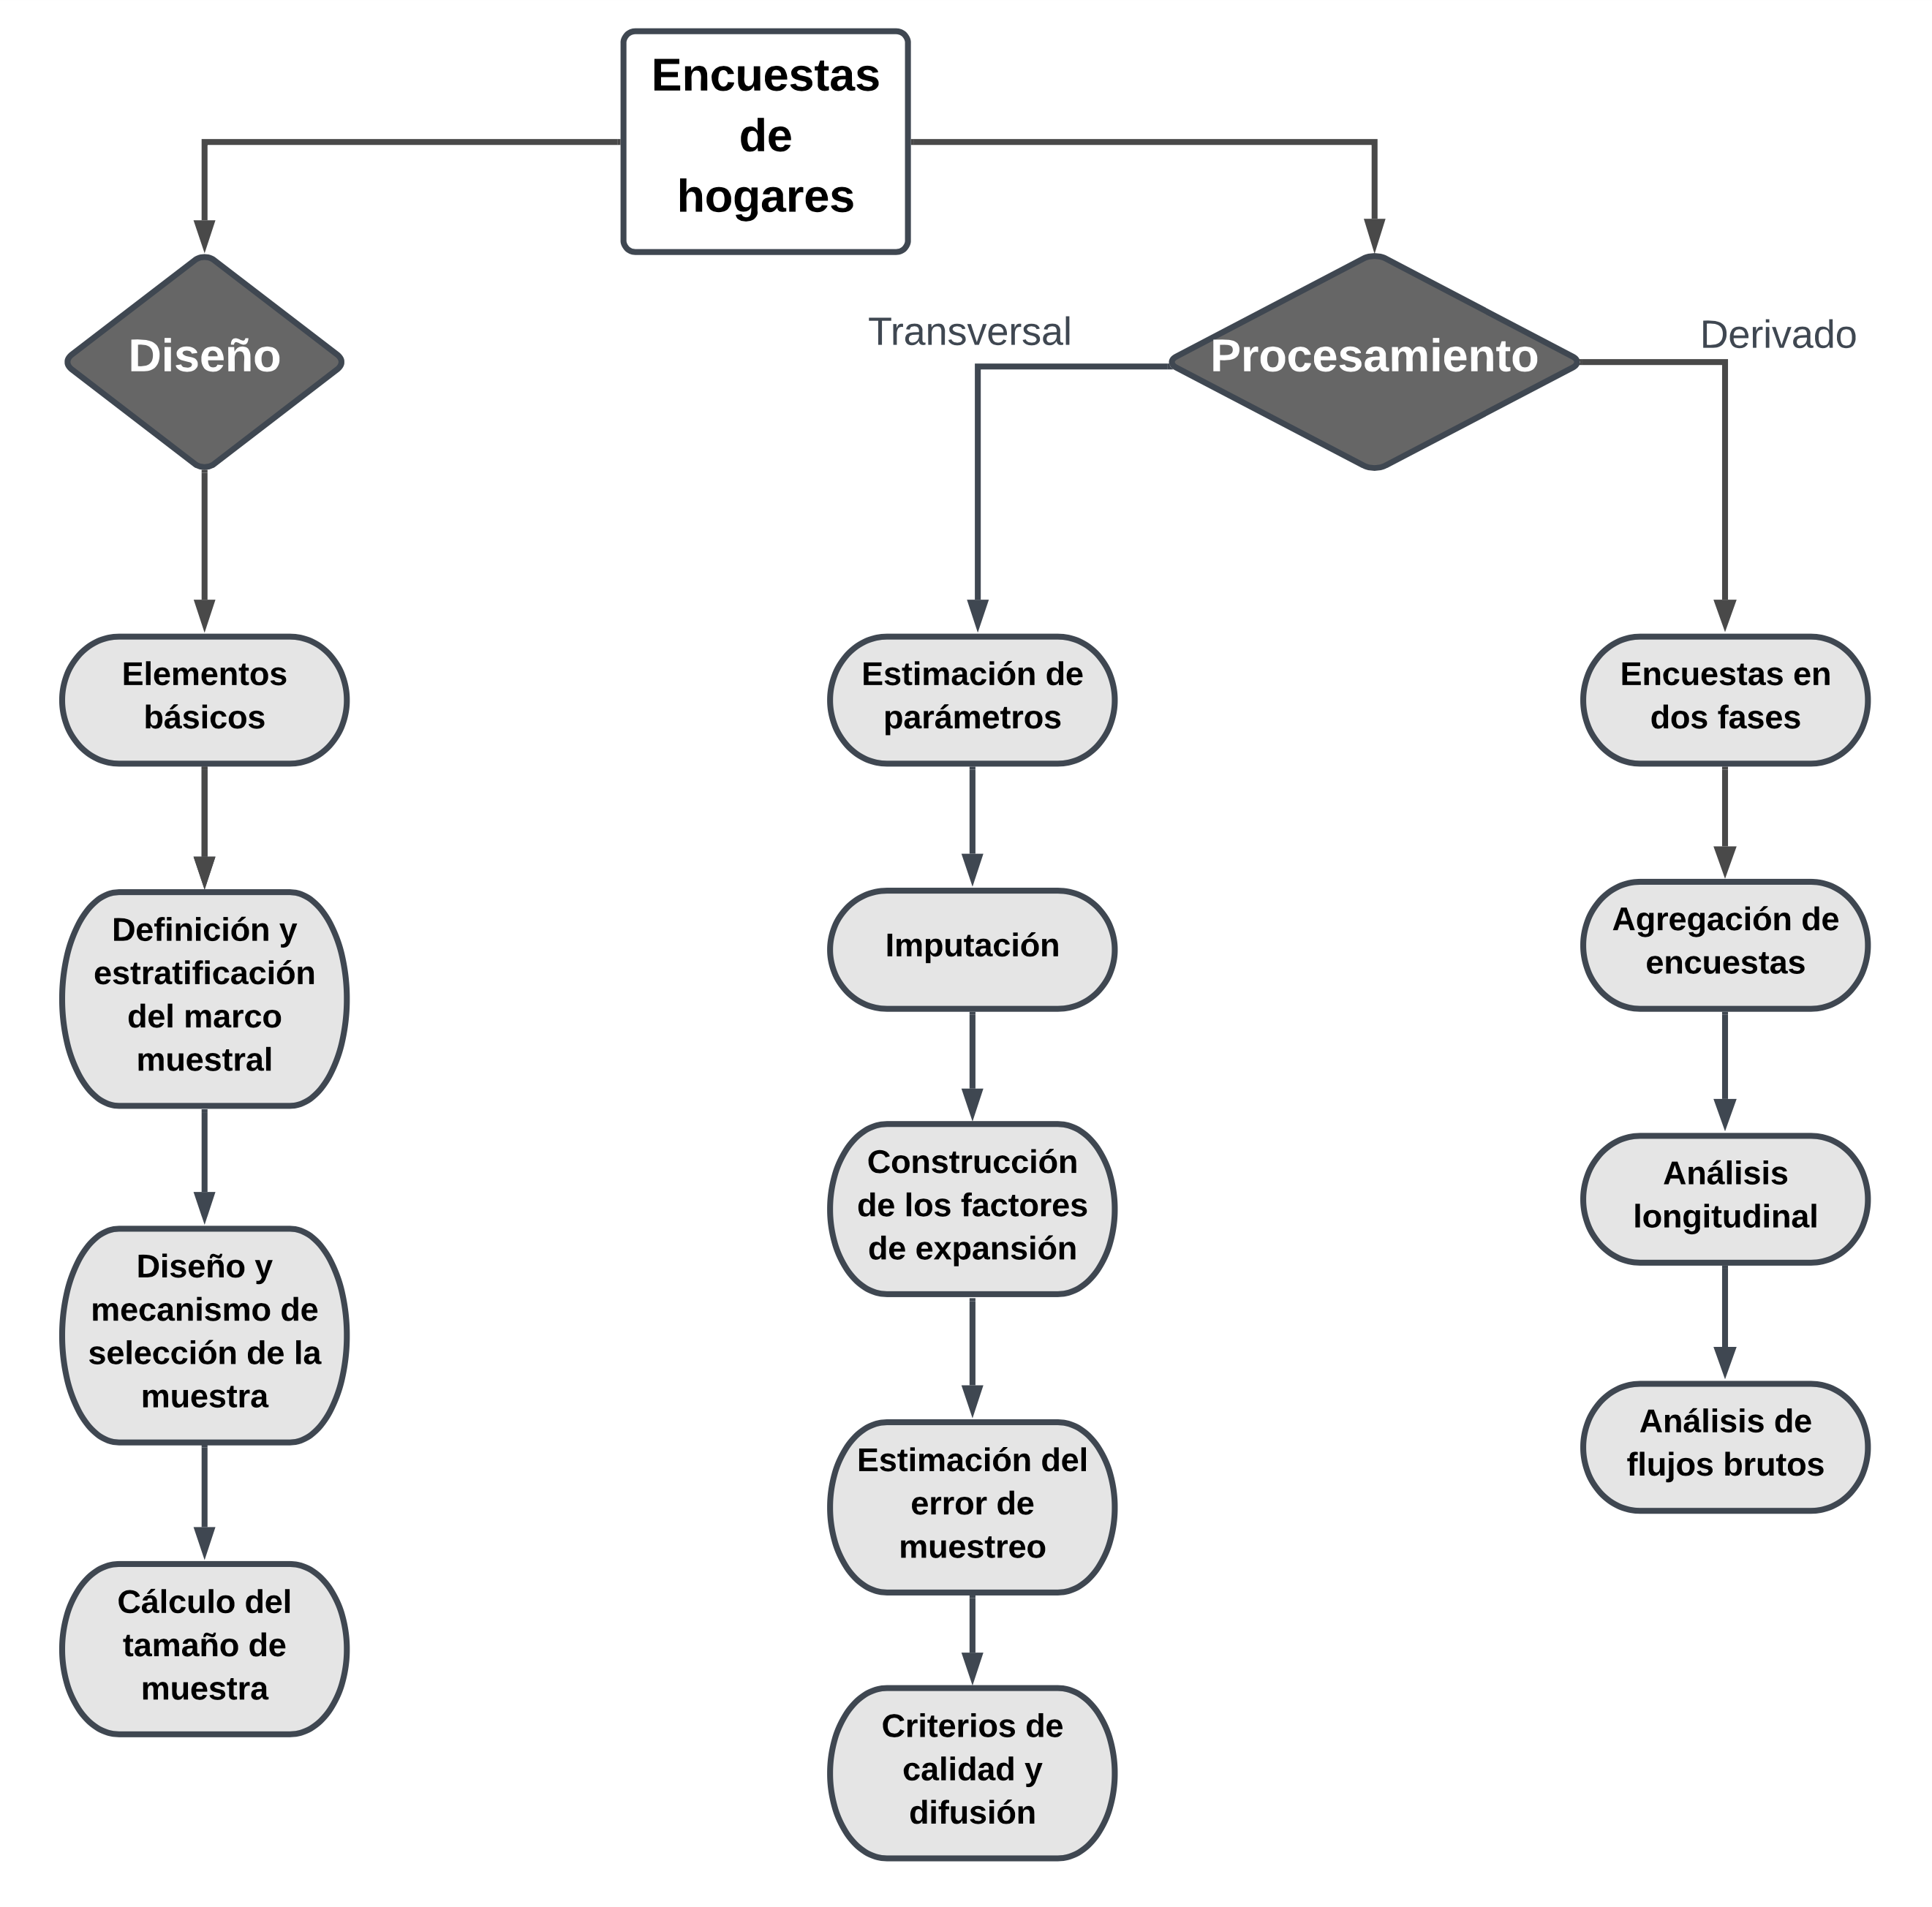
\includegraphics{Pics/Intro.png}
\caption{Esquema de procesos en el análisis y diseño de una encuesta de hogares.}
\end{figure}

En el primer capítulo se considera una breve introducción a la problemática de las encuestas de hogares. En el capítulo dos se aborda con más detalle los elementos básicos que se consideran por lo regular en los diseños de las encuestas de hogares. Un aspecto relevante de este documento es que, si bien considera que las encuestas de hogares tienen muchos elementos en común, diferencia de forma cuidadosa las particularidades de cada encuesta. Por ejemplo, en este capítulo se trata el tema del diseño de las encuestas rotativas y se profundiza en los diferentes parámetros que se pueden considerar en este tipo de operaciones; asimismo, describe las características metodológicas que se deben considerar al momento de diseñar la encuesta y revisa los conceptos esenciales que determinarán el tipo de aplicación que se debe considerar. El capítulo tres describe los principales diseños de muestreo que se utilizan en este tipo de estudios y expone de forma estándar los conceptos de estratificación y aglomeración de las poblaciones. El capítulo cuatro complementa estos conceptos con varias aplicaciones prácticas para determinar el tamaño de muestra adecuado para lograr los objetivos de la investigación. A pesar de que la literatura relacionada con la práctica del muestreo es relativamente abundante, existen pocos ejemplos prácticos que logren representar la problemática del tamaño de muestra y el lector podrá encontrar herramientas ilustrativas basadas en múltiples escenarios de la problemática social.

Pasando a la parte del análisis de las encuestas, el capítulo cinco revisa los procesos de imputación y ponderación en la encuesta. Los procesos de imputación tratan de recuperación tanta información como sea posible para que el investigador pueda contar con una base de datos rectangular y completa. Luego de esto, es necesario aplicar los factores de expansión a la información contenida en la base de datos para que se puedan realizar inferencias a nivel nacional o regional. Sin embargo, en aquellos casos en donde la imputación no resulta ser una técnica adecuada para completar la información faltante, es necesario realizar ajustes sistemáticos en los factores de expansión para que la muestra efectiva siga siendo una muestra representativa de toda la población. El capítulo seis analiza las principales metodologías de estimación, tanto de los parámetros de interés como de sus errores de muestreo. Si hay algo que distingue el análisis de las encuestas de cualquier otro tipo de estudio estadístico es que las propiedades importantes como insesgamiento, consistencia y eficiencia están basadas en el diseño de muestreo y no en supuestos metodológicos ligados a algún modelo estocástico. Es por esto que se presta especial atención a la estimación del error de muestreo, que no es otra cosa que una función de la varianza de las estimaciones, y se presentan las metodologías más comunes en términos de aproximaciones teóricas y computacionales al error de muestreo. El capítulo siete presenta de forma detallada los procesos que se surten cuando se agregan encuestas a lo largo de un periodo de tiempo. Acudiendo a la perspectiva del autor, el capítulo ocho presenta los criterios de calidad que se deberían tener en cuenta para decidir si una cifra, resultante de un proceso de estimación estadística basada en encuestas de hogares, debería ser o no publicada a la sociedad. Por úlitmo, el capítulo nueve presenta una discusión acerca del uso presente de las encuestas de hogares y los retos que depara el futuro en materia de la medición de indicadores sociales a través de las encuestas de hogares. Asimismo, en los anexos se contempla una revisión del software que se utiliza actualmente en los INE para llevar a cabo esta ardua tarea de diseñar y analizar las encuestas de hogares, una revisión rápida de algunas de las encuestas de la región, así como algunas directrices que se deberían considerar al momento de documentar los procesos asociados a las encuestas de hogares.

\hypertarget{referencias}{%
\chapter*{Referencias}\label{referencias}}
\addcontentsline{toc}{chapter}{Referencias}

  \bibliography{CEPAL.bib}

\end{document}
